\documentclass[conference]{IEEEtran}
\IEEEoverridecommandlockouts

\usepackage{cite}
\usepackage{amsmath,amssymb}
\usepackage{graphicx}
\usepackage{tikz}
\usetikzlibrary{arrows.meta,positioning,shapes.geometric}
\usepackage{booktabs}
\usepackage{url}

\graphicspath{{../benchmarks/}{./figures/}}

\newcommand{\taulow}{\tau_{\mathrm{low}}}
\newcommand{\tauhigh}{\tau_{\mathrm{high}}}
\newcommand{\sbar}{\bar{S}}

\begin{document}
\providecommand{\taulow}{\tau_{\mathrm{low}}}
\providecommand{\tauhigh}{\tau_{\mathrm{high}}}
\providecommand{\sbar}{\bar{S}}
\begin{figure}[t]
\centering
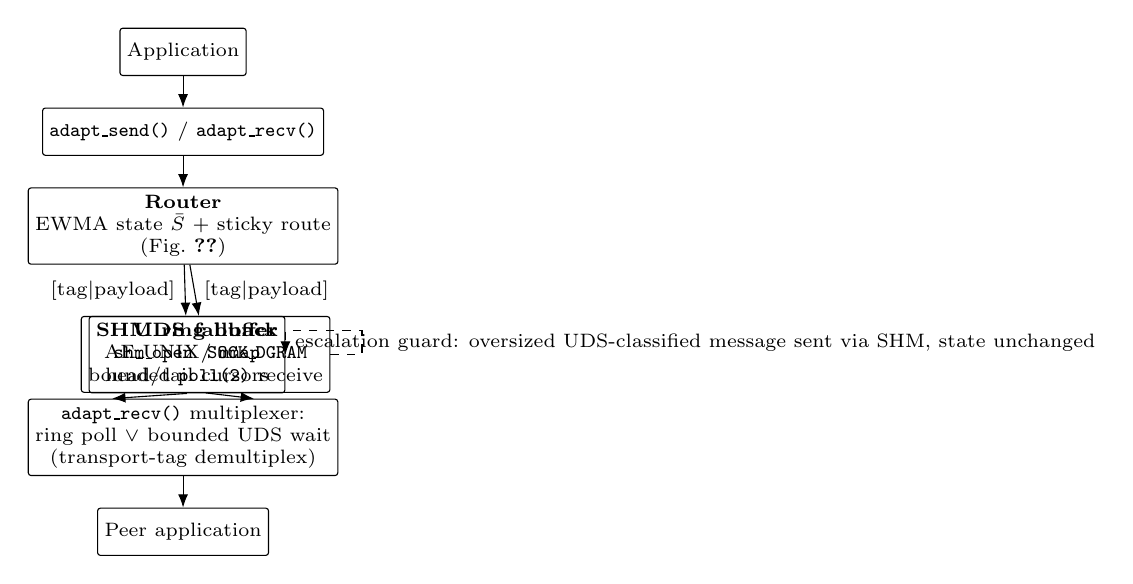
\begin{tikzpicture}[font=\scriptsize,>=Latex,node distance=4mm,
  box/.style={draw,rounded corners=1pt,align=center,minimum height=6mm,
              inner sep=2.5pt}]
\node[box] (app) {Application};
\node[box,below=4mm of app] (api)
  {\texttt{adapt\_send()} / \texttt{adapt\_recv()}};
\node[box,below=4mm of api] (rt)
  {\textbf{Router}\\ EWMA state $\sbar$ + sticky route\\ (Fig.~\ref{fig:decision})};
\node[box,below left=6.5mm and -13mm of rt.south] (shm)
  {\textbf{SHM ring buffer}\\ \texttt{shm\_open} / \texttt{mmap}\\
   head/tail cursors};
\node[box,below right=6.5mm and -13mm of rt.south] (uds)
  {\textbf{UDS fallback}\\ AF\_UNIX \texttt{SOCK\_DGRAM}\\ bounded
   \texttt{poll(2)} receive};
\node[box,below=17mm of rt] (mux)
  {\texttt{adapt\_recv()} multiplexer:\\ ring poll $\vee$ bounded UDS wait
   \\ (transport-tag demultiplex)};
\node[box,below=4mm of mux] (peer) {Peer application};
\draw[->] (app) -- (api);
\draw[->] (api) -- (rt);
\draw[->] (rt) -- (shm)
  node[midway,left,align=center]{[tag$\mid$payload]};
\draw[->] (rt) -- (uds)
  node[midway,right,align=center]{[tag$\mid$payload]};
\draw[->,dashed] (uds.east) -- ++(4mm,0) -- ++(0,3mm) -|
  node[pos=0.75,right,align=center]{escalation guard: oversized
  UDS-classified message sent via SHM, state unchanged}
  (shm.east);
\draw[->] (shm.south) -- ([xshift=-9mm]mux.north);
\draw[->] (uds.south) -- ([xshift=9mm]mux.north);
\draw[->] (mux) -- (peer);
\end{tikzpicture}
\caption{AdaptIPC data flow through one endpoint. Every outbound message is
classified by the EWMA/hysteresis router of Fig.~\ref{fig:decision} and
transmitted either through the lock-free shared-memory ring buffer or the
AF_UNIX datagram fallback; each frame carries a one-byte transport tag.
Dashed edge: the escalation guard sends an individual UDS-classified
message via SHM when it exceeds the datagram ceiling, without moving the
sticky routing state. On the receiving side, the
\texttt{adapt\_recv()} multiplexer accepts whichever transport delivers
next (Section~IV-D).}

\end{figure}
\end{document}

